\documentclass{beamer}
\beamertemplatenavigationsymbolsempty
\usecolortheme{beaver}
\setbeamertemplate{blocks}[rounded=true, shadow=true]
\setbeamertemplate{footline}[page number]
%
\usepackage[utf8]{inputenc}
\usepackage[english,russian]{babel}
\usepackage{amssymb,amsfonts,amsmath,mathtext}
\usepackage{subfig}
\usepackage[all]{xy} % xy package for diagrams
\usepackage{array}
\usepackage{multicol}% many columns in slide
\usepackage{hyperref}% urls
\usepackage{hhline}%tables
\usepackage{algpseudocode}
% Your figures are here:
\graphicspath{ {fig/} {../figures/} }

%----------------------------------------------------------------------------------------------------------
\title[\hbox to 56mm{Малоранговые разложения в распределенном обучении}]{Методы малоранговых разложений в распределенном и федеративном обучении}
\author[А.\,В. Ребриков]{Алексей Витальевич Ребриков}
\institute{Московский физико-технический институт}
\date{\footnotesize
\par\smallskip\emph{Курс:} Автоматизация научных исследований\par (практика, В.\,В.~Стрижов)/Группа 105
\par\smallskip\emph{Эксперт:} А.\,Н.~Безносиков
\par\smallskip\emph{Консультант:} А.\,В.~Зыль
\par\bigskip\small 2024}
%----------------------------------------------------------------------------------------------------------
\begin{document}
%----------------------------------------------------------------------------------------------------------
\begin{frame}
\thispagestyle{empty}
\maketitle
\end{frame}
%-----------------------------------------------------------------------------------------------------
% \begin{frame}{Цель исследования}
%\begin{block}{Решается задача}
%\end{block}
% \end{frame}
%-----------------------------------------------------------------------------------------------------

\newcommand{\R}{\mathbb{R}}
\newcommand{\cC}{\mathcal{C}}
\begin{frame}{Доклад с одним слайдом}
\begin{columns}[c]
\column{0.4\textwidth}
\begin{align*}
    \min \limits_{x \in \R^d} \left\{ f(x) = \frac{1}{n} \sum \limits_{i=1}^n f_i(x) \right\}
    \end{align*}

    \textbf{Ключевые пункты:}
    \begin{enumerate}
        \item Данные распределяются.
        \item Веса модели общие.
        \item Передача градиентов сжимается.
        \item Сжимается не сам градиент, а его разность. (EF21)
    \end{enumerate}

\column{0.6\textwidth}
\begin{figure}
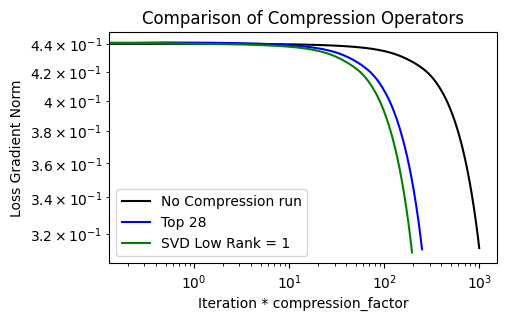
\includegraphics[width=1.0\textwidth]{output1.png}
\end{figure}\begin{figure}
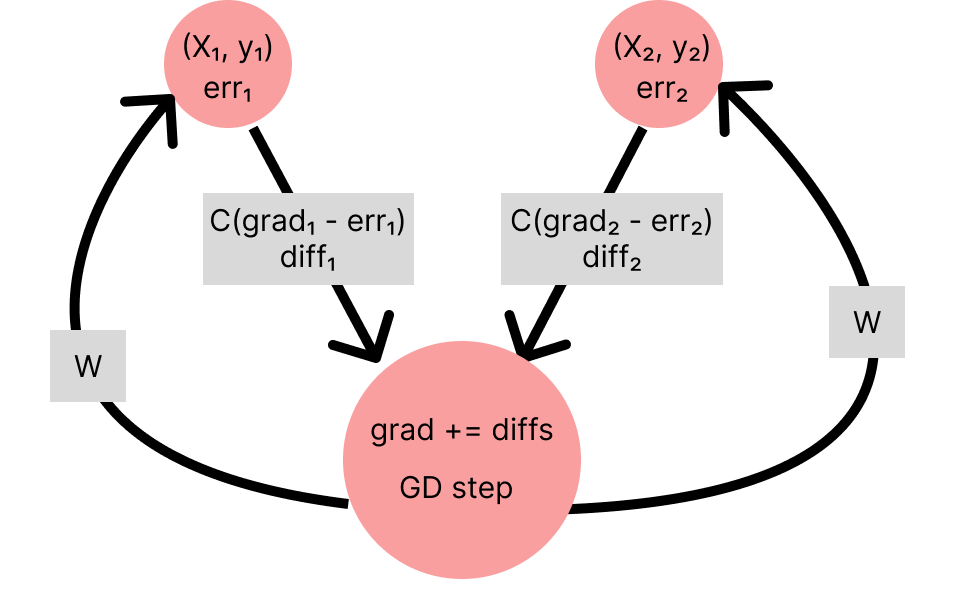
\includegraphics[width=0.8\textwidth]{img3.png}
\end{figure}

\end{columns}

\end{frame}


%----------------------------------------------------------------------------------------------------------
% \begin{frame}{Постановка задачи}
%
% \end{frame}
%----------------------------------------------------------------------------------------------------------
% \begin{frame}{Решение}
% \begin{columns}[c]
% \column{0.6\textwidth}
%     Столбец 1
% \column{0.4\textwidth}
%     Столбец 2
% \end{columns}
% \end{frame}
%----------------------------------------------------------------------------------------------------------
% \begin{frame}{Вычислительный эксперимент}
%
%  Что зритель видит на графике.
%
% \includegraphics[width=0.8\textwidth]{ErrorFunction}
%
% О чем говорит этот график.
%
% \end{frame}
%----------------------------------------------------------------------------------------------------------
% \begin{frame}{Заключение}
%     \begin{block}{Перечислите ваши результаты}
%     \begin{itemize}
%         \item предложен метод,
%         \item доказана теорема.
%     \end{itemize}
%     \end{block}
% \end{frame}
%----------------------------------------------------------------------------------------------------------

\end{document} 